\documentclass[12pt,a4paper]{article}

% Margins.
\setlength{\oddsidemargin}{0in}
\setlength{\evensidemargin}{0in}
\setlength{\headheight}{12pt}
\setlength{\headsep}{0pt}
\setlength{\topmargin}{-60pt}
\setlength{\textwidth}{6.5in}
\setlength{\textheight}{10.75in}

\usepackage{amsmath}
\usepackage{float}
\usepackage{graphicx}
\usepackage[hyphens]{url}
\usepackage{hyperref}	% Clickable links to figures, references and urls.
\usepackage{datetime}

% Drawing.
\usepackage{pgf}
\usepackage{tikz}

% Listings for formatting code.
\usepackage{listings}
\usepackage{textcomp}
% General options.
\lstset{breaklines=true, basicstyle=\small\ttfamily, tabsize=4, numbers=left, stepnumber=1, frame=single, showstringspaces=false, upquote=true}
% C++ specific high-lighting. Comments are 50/50 shades of green/black and strings coloured with 60/40 red/black mixture.
\lstset{language=[ISO]C++, commentstyle=\color{green!50!black}, keywordstyle=\color{blue}, stringstyle=\color{red!60!black}}

%opening
\title{Programming for Engineers I\\Class 07\\Functions, Pointers and Arrays}
\author{Attique Dawood}
\date{July 08, 2014\\[0.2cm] Last Modified: \today, \currenttime}
\begin{document}
\maketitle
\section{Announcements}
\begin{itemize}
\item None.
\end{itemize}
\section{Revision}
\begin{itemize}
\item Bubblesort.
\item 2D arrays.
\end{itemize}
\section{Functions}
Functions are like subtasks. They receive some information, do some process and provide a result. Functions are invoked through a calling program. Calling program does not need to know what the function is doing and how it is performing its task. There is a specific function-calling methodology. The calling program calls a function by giving it some information and receives the result.

We have a \verb|main()| in every C program. \verb|main()| is also a function. When we write a function, it must start with a name, parentheses, and surrounding braces just like with \verb|main()|. Functions are very important in code reusing.

There are two categories of functions:

\begin{description}
\item [1]Functions that return a value
\item [2]Functions that do not return a value
\end{description}

Suppose, we have a function that calculates the square of an integer such that function will return the square of the integer. Similarly we may have a function which displays some information on the screen so this function is not supposed to return any value to the calling program.
\subsection{Structure of a Function}
The declaration syntax of a function is as follows:\\[0.3cm]
\textit{return-value-type    function-name( argument-list )\\
$\left\lbrace\right.$\\
\hspace{1cm}declarations and statements\\
$\left.\right\rbrace$}
\begin{lstlisting}
#include <iostream>
using namespace std;

// Function definition/implementation.
void Display()
{
	cout << "Hello" << endl;
}

int main()
{
	Display(); // Function call	
	
	return 0;
}
\end{lstlisting}
\begin{lstlisting}
//This function calculates the square of a number and returns it.
#include <iostream>
using namespace std;

int square(int number)
{
    int result = 0;
    result = number * number;
    return result;
}

void main()
{
    int number, result;
    result = 0;
    number = 0;
    // Getting the  input from the user
    cout << "Please enter the number to calculate the square: ";
    cin >> number;

    // Calling the function square(int number)
    result = square(number);
    cout << "The square of " << number << " is " << result << endl;
}
\end{lstlisting}
\subsection{Advantages of using Functions:}
\begin{itemize}
\item Code Reusability
\item Modularity
\item Readability
\end{itemize}
\section{Exiting a Function}
\begin{itemize}
\item To terminate a function that returns a value use the statement \verb|return somevalue;|.
\item To exit a function that doesn't return a value simply use \verb|return;|
\item This is similar to \verb|break|. A function will immediately exit on \verb|return| statement.
\end{itemize}
\section{Recursive Functions}
\begin{itemize}
\item Recursive functions call themselves.
\item There must be a terminating condition for recursive functions.
\item \textbf{Interesting Fact:} You can call \verb|main()| in \verb|main()| function! This will put your program in a loop. Although not really a good programming practice but it does give a convenient way to test your program when you don't want to re-run the exe.
\end{itemize}
\begin{lstlisting}[caption={Recursive Factorial Function}]
#include <iostream>
using namespace std;

// Function definition/implementation.
int Factorial(int n)
{
	if (n == 0 || n == 1)
	{
		return 1;
	}
	return (Factorial(n-1) * n);
}

int main()
{
	int k;
	cout << "Enter a number to calculate factorial: ";
	cin >> k;
	cout << "Factorial of " << k << " = " << Factorial(k) << endl;
	
	return 0;
}
\end{lstlisting}
\section{Pointers}
\begin{itemize}
\item Pointers are very special variables that let you manipulate other `normal' variables (int, float, double etc.).
\item A pointer stores the address of the variable it wants to access (manipulate).
\item Pointer declaration requires declaration of the type of variable that pointer will `point' to. \verb|int* xp| means a pointer named `xp' that can point to an integer variable.
\item Accessing the value of `pointed' variable is called `dereferencing' the pointer. This is done by using a \verb|*| with pointer. Example: \verb|Display: cout << *xp;|, \verb|Input: cin >> *xp;|
\item \textbf{Remember, like other variables, a pointer will contain garbage if it is not initialised with the address of a valid variable}.
\item \textbf{Any attempt to access an invalid address stored in pointer will likely result in runtime crash}.
\item Pointers allow dynamic memory access and is probably the most powerful feature in C. Mastering the use of pointers can result in efficient and faster programs.
\item Basic pointer usage is essential for understanding dynamic memory allocation/deallocation.
\end{itemize}
\begin{lstlisting}[caption={Pointer Basics}]
#include <iostream>
using namespace std;

int main()
{
	int x = 34;
	int* xp; // Pointer declaration.
	xp = &x; // Pointer 'xp' initialised with address of x.
	
	cout << "Value of x: " << x << endl; // Value stored in x.
	cout << "Address of x: " << &x << endl; // Address of x in memory.
	cout << "Value of xp: " << xp << endl; // xp stores address of x.
	cout << "Value of x using xp: " << *xp << endl; // Display value stored in x using pointer xp.
	*xp = -1; // Change value stored in x using pointer xp.
	cout << "New value of x: " << endl
		 << "Using x: " << x << endl
		 << "Using xp: " << *xp << endl; 
	
	return 0;
}
\end{lstlisting}
\section{Pointer Arithmetic}
\begin{itemize}
\item Pointers can be incremented or decremented.
\item If a pointer is incremented by one then the value of address it stores is incremented by the size of data type.
\item Example: An int pointer contains 10. If it is incremented then the new value is 14 because size of int is 4.
\item This makes sense when viewed from the perspective of array access. In an int array each location occupies 4 bytes. The address of each location is separated by 4 bytes. To access 3rd element \verb|*(array+2)| is used. If first address is at 0 then second would be at 4 and third at 8.
\end{itemize} 
\begin{lstlisting}[caption={Pointer Arithmetic}]
#include <iostream>
using namespace std;

int main()
{
	int Array[5] = {3,7,2,1,5};
	int* pA;
	pA = Array; // pA stores starting address of Array.
	
	for (int i=0; i<5; i++)
	{
		cout << *pA << endl;
		pA++; // Increment pointer.
	}

	return 0;
}
\end{lstlisting}
\section{Pointers and Arrays}
The name of array is the pointer to its first element. A subscript besides array name can be translated in english as, ``access element located this much distance from start.'' Keep in mind that \verb|Array[i]| is the same as \verb|*(Array+i)| which means that you only need array pointer to access array elements using the subscript. Consider the following code
\begin{lstlisting}[caption={Arrays and Pointers}]
#include <iostream>
using namespace std;

int Area(int*, int*); // Function prototype.

int main()
{
	int Array[5] = {3,7,2,1,5};

	cout << Array << endl; // Prints the address of array.

	// Using subscript.
	cout << Array[0] << endl; // Print the value of element located a distance of 0 from start.
	cout << Array[3] << endl; // Print the value of element located a distance of 3 from start.
	cout << Array[5] << endl; // Print the value of element located a distance of 5 from start. ERROR! Out of bound.

	// Using Pointers.
	cout << *(Array+0) << endl; // Prints the value of first element which is 3.
	cout << *(Array+1) << endl; // Prints the value of second element which is 7.
	cout << *(Array+5) << endl; // Prints the value of sixth element which out of bound or ERROR.

	return 0;
}
\end{lstlisting}
\begin{figure}[H]
\centering
\begin{tikzpicture}
	% Writing 'Array'
	\coordinate [label=left:\textsf{Array Pointer (\texttt{Array})}] (Arraypointer) at (-1.5cm,0.3cm);
	\draw[thick, ->, >=stealth] (-1.5cm, 0.3cm) -- (0cm, 0.3cm);
	% Drawing boxes.
	\foreach \x in {0.0cm, 1.0cm, 2.0cm, 3.0cm, 4.0cm}
		\draw[thick] (\x, 0cm) rectangle (\x+1.0cm, 0.6cm);
	% Writing numbers in boxes. This is original array.
	\foreach \x/\y in {0.0cm/3, 1.0cm/7, 2.0cm/2, 3.0cm/1, 4.0cm/5}
		\draw (\x+0.5cm,0.3cm) node {\texttt{\y}};
	\def\XD{0cm}
	\def\YD{-0.5cm}
	% Drawing an arrow and pointer.
	\coordinate [label=left:\texttt{Array[0] or *(Array+0)}] (Array0) at (-1cm,\YD);
	\draw[thick, ->, >=stealth] (-1cm, \YD) -- (0cm+\XD, \YD);
	\draw[dashed] (\XD,0cm) -- (\XD,\YD-0.5);
	\draw[dashed] (\XD,\YD-0.3cm) rectangle (\XD+1cm,\YD+0.3cm);

	\def\XD{1cm}
	\def\YD{-1cm}
	% Drawing an arrow and pointer.
	\coordinate [label=left:\texttt{Array[1] or *(Array+1)}] (Array1) at (-1cm,\YD);
	\draw[thick, ->, >=stealth] (-1cm, \YD) -- (0cm+\XD, \YD);
	\draw[dashed] (\XD,0cm) -- (\XD,\YD-0.5);
	\draw[dashed] (\XD,\YD-0.3cm) rectangle (\XD+1cm,\YD+0.3cm);

	\def\XD{2cm}
	\def\YD{-1.5cm}
	% Drawing an arrow and pointer.
	\coordinate [label=left:\texttt{Array[2] or *(Array+2)}] (Array2) at (-1cm,\YD);
	\draw[thick, ->, >=stealth] (-1cm, \YD) -- (0cm+\XD, \YD);
	\draw[dashed] (\XD,0cm) -- (\XD,\YD-0.5);
	\draw[dashed] (\XD,\YD-0.3cm) rectangle (\XD+1cm,\YD+0.3cm);

	\def\XD{3cm}
	\def\YD{-2cm}
	% Drawing an arrow and pointer.
	\coordinate [label=left:\texttt{Array[3] or *(Array+3)}] (Array3) at (-1cm,\YD);
	\draw[thick, ->, >=stealth] (-1cm, \YD) -- (0cm+\XD, \YD);
	\draw[dashed] (\XD,0cm) -- (\XD,\YD-0.5);
	\draw[dashed] (\XD,\YD-0.3cm) rectangle (\XD+1cm,\YD+0.3cm);
	
	\def\XD{4cm}
	\def\YD{-2.5cm}
	% Drawing an arrow and pointer.
	\coordinate [label=left:\texttt{Array[4] or *(Array+4)}] (Array4) at (-1cm,\YD);
	\draw[thick, ->, >=stealth] (-1cm, \YD) -- (0cm+\XD, \YD);
	\draw[dashed] (\XD,0cm) -- (\XD,\YD-0.5);
	\draw[dashed] (\XD,\YD-0.3cm) rectangle (\XD+1cm,\YD+0.3cm);
	
	\def\XD{5cm}
	\def\YD{-3cm}
	% Drawing an arrow and pointer.
	\coordinate [label=left:\texttt{Array[5] or *(Array+5)}] (Array5) at (-1cm,\YD);
	\draw[thick, ->, >=stealth] (-1cm, \YD) -- (0cm+\XD, \YD);
	\draw[dashed] (\XD,0cm) -- (\XD,\YD-0.5);
	\coordinate [label=right:\texttt{ERROR!}] (Error) at (\XD,\YD);
\end{tikzpicture}
\caption{Using pointer to access array elements}
\label{Array-pointer-element-access}
\end{figure}
\section{Passing By Value and By Reference}
\begin{itemize}
\item Basic data types are always passed by value to functions. A `local' copy of variable is created in function and used.
\item Extra variables created in function may take up sizeable memory if there are many input arguments. Large arrays if passed as copy can create problems.
\item Variables can be passed as reference by specifying a preceding \verb|&| with variable name. \textbf{There is no change in function call}.
\end{itemize}
\begin{lstlisting}[caption={Passing Function Arguments as Reference}]
//This function calculates the square of a number and returns it.
#include <iostream>
using namespace std;

int sum(int& A, int& B)
{
    int result = A+B;
    return result;
}

void main()
{
    int x = 3;
    int y = 7;
    
    cout << sum(x, y) << endl;
    
    return 0;
}
\end{lstlisting}
\section{Memory Map in a Normal Function Call}
Consider the code in listing 1. Before the function call on line 8 the memory will contain three variable a, b and c. Inside the function, three additional variables, x, y and z, will be created. Values of a and b will be copied into x and y as these are the function arguments. After the function call ends, value of z, which is 15, will be copied onto c. Variables x, y and z will be destroyed or deallocated after function call. Figure \ref{A-Normal-Function-Call} gives a picture of exactly how this happens.
\begin{lstlisting}[caption={Calling a function}]
#include <cstdio>
int Area(int, int); // Function prototype.
int main()
{
	int a, b, c;
	a = 3;
	b = 5;
	c = Area(a, b); // Function call.
	
	return 0;
}
// Function definition.
int Area(int x, int y)
{
	int z;
	z = x*y;
	return z;
}
\end{lstlisting}
\begin{figure}[H]
\centering
\begin{tikzpicture}
	% Drawing main()
	\coordinate [label=above:\texttt{main()}] (main) at (0.6cm,0cm);
	\draw (0cm,0cm) rectangle (3cm,-3.5cm);
	\coordinate [label=right:\texttt{int a, b, c;}] (intabc) at (0.1cm,-0.5cm);
	\coordinate [label=right:\texttt{a=3;}] (a3) at (0.1cm,-1cm);
	\coordinate [label=right:\texttt{b=5;}] (b5) at (0.1cm,-1.5cm);
	\coordinate [label=right:\texttt{c=Area(a, b);}] (carea) at (0.1cm,-2cm);
	\coordinate [label=right:\texttt{return 0;}] (return0) at (0.1cm,-3cm);

	% Drawing Area() function.
	\coordinate [label=above:\texttt{int Area(int x, int y)}] (main) at (7cm,0cm);
	\draw (5cm,0cm) rectangle (8cm,-2cm);
	\coordinate [label=right:\texttt{int z;}] (intz) at (5.1cm,-0.5cm);
	\coordinate [label=right:\texttt{z = x*y;}] (zxy) at (5.1cm,-1cm);
	\coordinate [label=right:\texttt{return z;}] (return z) at (5.1cm,-1.5cm);

	% Drawing arrows
	\coordinate [label=above:1] (1) at (-0.2cm,-0.5cm);
	\draw[thick, ->, >=stealth] (-0.2cm, -0.5cm) -- (-0.2cm, -2cm);
	\coordinate [label=above:2] (2) at (4cm,-1.2cm);
	\draw[thick, ->, >=stealth] (3.1cm, -2cm) -- (4.9cm, -0.5cm);
	\coordinate [label=above:3] (3) at (4cm,-2.3cm);
	\draw[thick, ->, >=stealth] (4.9cm, -1.5cm) -- (3.2cm, -2cm);
	
	% Drawing Memory Map.
	\coordinate [label=right:\texttt{Memory Before 2}] (Memory1) at (0cm,-4.2cm);
	\draw (0cm,-4.5cm) rectangle (3cm,-5cm);
	\coordinate [label=above:\texttt{a=3}] (a3) at (1.5cm,-5cm);
	\draw (0cm,-5cm) rectangle (3cm,-5.5cm);
	\coordinate [label=above:\texttt{b=5}] (b5) at (1.5cm,-5.5cm);
	\draw (0cm,-5.5cm) rectangle (3cm,-6cm);
	\coordinate [label=above:\texttt{c=XXX}] (cXXX) at (1.5cm,-6cm);
	
	\coordinate [label=right:\texttt{Memory Before 3}] (Memory2) at (5cm,-4.2cm);
	\draw (5cm,-4.5cm) rectangle (8cm,-5cm);
	\coordinate [label=above:\texttt{a=3}] (a3) at (6.5cm,-5cm);
	\draw (5cm,-5cm) rectangle (8cm,-5.5cm);
	\coordinate [label=above:\texttt{b=5}] (b5) at (6.5cm,-5.5cm);
	\draw (5cm,-5.5cm) rectangle (8cm,-6cm);
	\coordinate [label=above:\texttt{c=XXX}] (cXXX) at (6.5cm,-6cm);
	\draw (5cm,-6cm) rectangle (8cm,-6.5cm);
	\coordinate [label=above:\texttt{x=3}] (x3) at (6.5cm,-6.5cm);
	\draw (5cm,-6.5cm) rectangle (8cm,-7cm);
	\coordinate [label=above:\texttt{y=5}] (y5) at (6.5cm,-7cm);
	\draw (5cm,-5cm) rectangle (8cm,-7.5cm);
	\coordinate [label=above:\texttt{z=15}] (z15) at (6.5cm,-7.5cm);
	
	\coordinate [label=right:\texttt{Memory After 3}] (Memory3) at (0cm,-7.2cm);
	\draw (0cm,-7.5cm) rectangle (3cm,-8cm);
	\coordinate [label=above:\texttt{a=3}] (a3) at (1.5cm,-8cm);
	\draw (0cm,-8cm) rectangle (3cm,-8.5cm);
	\coordinate [label=above:\texttt{b=5}] (b5) at (1.5cm,-8.5cm);
	\draw (0cm,-8.5cm) rectangle (3cm,-9cm);
	\coordinate [label=above:\texttt{c=15}] (c15) at (1.5cm,-9cm);
\end{tikzpicture}
\caption{A normal function call}
\label{A-Normal-Function-Call}
\end{figure}
\section{Passing by Reference}
If function arguments are passed--by--reference then the function arguments directly refer to the original variables. New variables are not created. If the value of function arguments is changed then the value of original arguments is also varied. Syntax for passing variables by reference is giving in code listing 2.
\begin{lstlisting}[caption={Passing by reference}]
#include <cstdio>
int Area(int&, int&); // Function prototype.
int main()
{
	int a, b, c;
	a = 3;
	b = 5;
	c = Area(a, b); // Function call.
	
	return 0;
}
// Function definition.
int Area(int& x, int& y)
{
	int z = x*y;
	x=7;
	return z;
}
\end{lstlisting}
\begin{figure}[H]
\centering
\begin{tikzpicture}
	% Drawing main()
	\coordinate [label=above:\texttt{main()}] (main) at (0.6cm,0cm);
	\draw (0cm,0cm) rectangle (3cm,-3.5cm);
	\coordinate [label=right:\texttt{int a, b, c;}] (intabc) at (0.1cm,-0.5cm);
	\coordinate [label=right:\texttt{a=3;}] (a3) at (0.1cm,-1cm);
	\coordinate [label=right:\texttt{b=5;}] (b5) at (0.1cm,-1.5cm);
	\coordinate [label=right:\texttt{c=Area(a, b);}] (carea) at (0.1cm,-2cm);
	\coordinate [label=right:\texttt{return 0;}] (return0) at (0.1cm,-3cm);

	% Drawing Area() function.
	\coordinate [label=above:\texttt{int Area(int\& x, int\& y)}] (main) at (7.2cm,0cm);
	\draw (5cm,0cm) rectangle (8cm,-2cm);
	\coordinate [label=right:\texttt{int z = x*y;}] (zxy) at (5.1cm,-0.5cm);
	\coordinate [label=right:\texttt{x=7;}] (x7) at (5.1cm,-1cm);
	\coordinate [label=right:\texttt{return z;}] (return z) at (5.1cm,-1.5cm);

	% Drawing arrows
	\coordinate [label=above:1] (1) at (-0.2cm,-0.5cm);
	\draw[thick, ->, >=stealth] (-0.2cm, -0.5cm) -- (-0.2cm, -2cm);
	\coordinate [label=above:2] (2) at (4cm,-1.2cm);
	\draw[thick, ->, >=stealth] (3.1cm, -2cm) -- (4.9cm, -0.5cm);
	\coordinate [label=above:3] (3) at (4cm,-2.3cm);
	\draw[thick, ->, >=stealth] (4.9cm, -1.5cm) -- (3.2cm, -2cm);
	
	% Drawing Memory Map.
	\coordinate [label=right:\texttt{Memory Before 2}] (Memory1) at (0cm,-4.2cm);
	\draw (0cm,-4.5cm) rectangle (3cm,-5cm);
	\coordinate [label=above:\texttt{a=3}] (a3) at (1.5cm,-5cm);
	\draw (0cm,-5cm) rectangle (3cm,-5.5cm);
	\coordinate [label=above:\texttt{b=5}] (b5) at (1.5cm,-5.5cm);
	\draw (0cm,-5.5cm) rectangle (3cm,-6cm);
	\coordinate [label=above:\texttt{c=XXX}] (cXXX) at (1.5cm,-6cm);
	
	\coordinate [label=right:\texttt{Memory Before 3}] (Memory2) at (5cm,-4.2cm);
	\draw (5cm,-4.5cm) rectangle (8cm,-5cm);
	\coordinate [label=above:\texttt{a,x=7}] (a3) at (6.5cm,-5cm);
	\draw (5cm,-5cm) rectangle (8cm,-5.5cm);
	\coordinate [label=above:\texttt{b,y=5}] (b5) at (6.5cm,-5.5cm);
	\draw (5cm,-5.5cm) rectangle (8cm,-6cm);
	\coordinate [label=above:\texttt{c=XXX}] (cXXX) at (6.5cm,-6cm);
	\draw (5cm,-6cm) rectangle (8cm,-6.5cm);
	\coordinate [label=above:\texttt{z=15}] (z15) at (6.5cm,-6.5cm);
	
	\coordinate [label=right:\texttt{Memory After 3}] (Memory3) at (0cm,-7.2cm);
	\draw (0cm,-7.5cm) rectangle (3cm,-8cm);
	\coordinate [label=above:\texttt{a=7}] (a3) at (1.5cm,-8cm);
	\draw (0cm,-8cm) rectangle (3cm,-8.5cm);
	\coordinate [label=above:\texttt{b=5}] (b5) at (1.5cm,-8.5cm);
	\draw (0cm,-8.5cm) rectangle (3cm,-9cm);
	\coordinate [label=above:\texttt{c=15}] (c15) at (1.5cm,-9cm);
\end{tikzpicture}
\caption{A referenced function call}
\label{A-Referenced-l-Function-Call}
\end{figure}
\section{Using Pointers for Referencing}
Since pointers point to original variables they can be used to change the value of original variables in a function call.
\begin{lstlisting}[caption={Pointers as Arguments}]
#include <cstdio>
int Area(int*, int*); // Function prototype.
int main()
{
	int a, b, c;
	a = 3;
	b = 5;
	c = Area(&a, &b); // Function call by address.
	
	return 0;
}
// Function definition.
int Area(int* x, int* y)
{
	int z = (*x)*(*y); // Dereferencing pointers.
	*x=7; // Changes value of a in main().
	return z;
}
\end{lstlisting}
\section{Passing Arrays in Functions}
\begin{itemize}
\item Arrays are always passed as reference to functions.
\item There are two syntax used for array passing; subscript and pointer.
\end{itemize}
\begin{lstlisting}[caption={Passing Array Using Subscript Notation}]
#include <iostream>
using namespace std;

void DisplayArray(int [], const int); // Function prototype.

int main()
{
	cont int SIZE = 5;
	int testarray[SIZE] = {2,3,4,2,1};
	DisplayArray(testarray, SIZE); // Function call.
	
	return 0;
}

void DisplayArray(int test[], const int size)
{
	for (int i=0; i<size; i++)
		cout << test[i] << endl;
}
\end{lstlisting}
\begin{lstlisting}[caption={Passing Array Using Pointer Notation}]
#include <iostream>
using namespace std;

void DisplayArray(int*, const int); // Function prototype.

int main()
{
	cont int SIZE = 5;
	int testarray[SIZE] = {2,3,4,2,1};
	DisplayArray(testarray, SIZE); // Function call.
	
	return 0;
}

void DisplayArray(int* test, const int size)
{
	for (int i=0; i<size; i++)
		cout << test[i] << endl;
}
\end{lstlisting}
\end{document}